\documentclass[a4paper]{article}
\usepackage[a4paper, total={6in, 9in}]{geometry}
\usepackage{amsmath}
\usepackage{csvsimple}
\usepackage{graphicx}
\usepackage{siunitx}
\usepackage{float}
\usepackage{subcaption}
\usepackage{blindtext}

\graphicspath{ {./img/} }

\title{Laboration i Geometrisk Optik}

\author{Emil Babayev}
\date{2020-03-27}
\begin{document}
\maketitle

\section{Inledning}
\subsection{Introduktion och sammanfattning}

\subsection{Introduktionsuppgifter}
För uppgift 1, se appendix A om kollimering och linjering. 
Uppgift 2 beskrivs här nedan.
Använder formlen för minimiavlänkning, ekvation \ref{eq: avl}, där $n$ är brytningsindex i materialet, $\delta$ är avlänkningsvinkeln och 
$\alpha$ är vinkeln mellan de brytande ytorna i prismat.
\begin{equation}
    \label{eq: avl}
    n = \frac{sin(\frac{\delta +\alpha}{2})}{sin(\frac{\alpha}{2})}
\end{equation}
och löser ut $\delta$, som vi söker. Detta ger ekvation \ref{eq: avl2}:
\begin{equation}
    \label{eq: avl2}
    \delta = 2 arcsin(n sin(\frac{\alpha}{2})) - \alpha
\end{equation}
Insättning av $n=1.57$ och $\alpha = \ang{60}$ ger $\delta = \ang{43.44}$.

\section{Teori}
\subsection{Divergens hos en stråle}
Divergensen hos en ljuskälla definieras som vinkeln hos ljuskonen som bildas när ljuset propagerar. Divergensvinkeln $\theta$ kan beräknas med ekvation \ref{eq: div}:
\begin{equation}
    \theta = 2 arctan(\frac{d_1 - d_2}{2l})
    \label{eq: div}
\end{equation}
Sambandet kan härledas om man iakttar en del av ljuskonen som är långt borta från alla fokus och utför lite trigonometri. Se figur \ref{fig:divergens}. $d_1$ och $d_2$
är ljuskonens diameter i två punkter, och $l$ är avståndet där emellan.  
\begin{figure}[h!]
    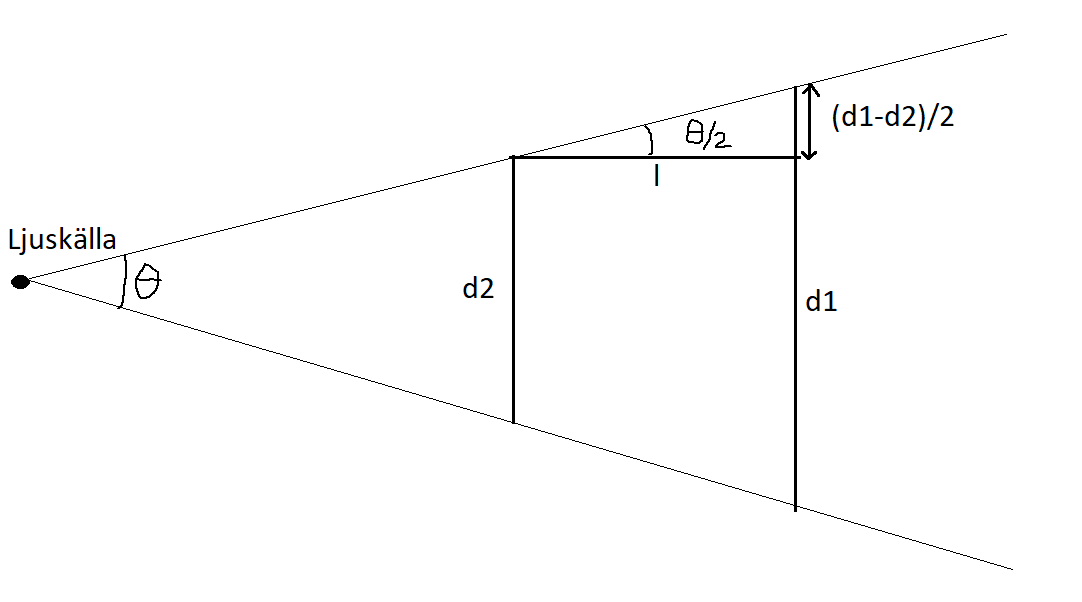
\includegraphics[width=0.6\textwidth]{divergens}
    \caption{Härledning av divergensvinkel}
    \label{fig:divergens}
\end{figure}
\pagebreak
\subsection{Optiska komponenter}
De optiska komponenter som används i laborationen är prisman och konvexa linser.
\subsubsection{Prismor}
Prismat är en komponent med platta genomskinliga ytor där ljuset kan passera. Vi tittar på triangulära prismor i denna laboration,
där varje gränsyta följer Snells brytningslag, ekvation \ref{eq:brytning}. $n$ brytningsindex. $\alpha$ infalls-/brytningsvinkel.
\begin{equation}
    n_1*sin(\alpha_1) = n_2*sin(\alpha_2)
    \label{eq:brytning}
\end{equation}
Varje gång en ljusstråle passerar igenom en gränsyta bryts det. I vårt fall bryts det mot normalen när det äntrar prismat, eftersom prismat är av glas och vi antar luft utanför.
När det sedan lämnar prismat bryts det bort från normalen. Detta resulterar i att ljuset böjs av en viss vinkel jämfört med den ursprungliga riktningen. Denna vinkel kallas
avlänkningsvinkeln, som vi betecknar med $\delta$. Den brytande kanten får också en egen vinkel, $\alpha$. Se figur \ref{fig:prism}.
\begin{figure}[h!]
    \centering
    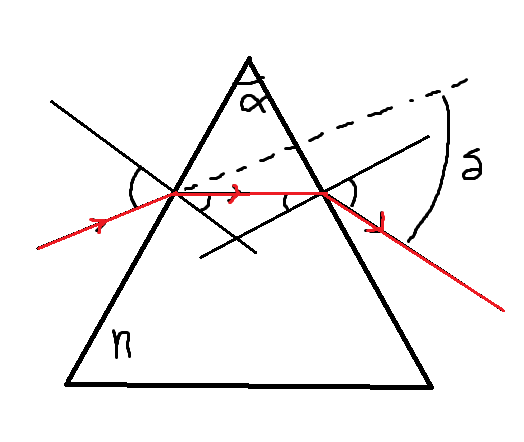
\includegraphics[width=0.5\textwidth]{prism.png}
    \caption{Principskiss av prisma. Strålgången är markerad i rött.}
    \label{fig:prism}
\end{figure}
Avlänkningsvinkeln blir minst då strålgången är symmetrisk kring prismat. Det finns en formel för minsta avlänkningsvinkel, ekvation \ref{eq:avlankning}.
\begin{equation}
    n = \frac{sin(\frac{\delta +\alpha}{2})}{sin(\frac{\alpha}{2})}
    \label{eq:avlankning}
\end{equation}

\subsubsection{Linser}
Linserna vi pratar om i laborationen är två sfäriska, sammanfogade gränsytor som buktar utåt (konvexa). Även i linser gäller 
Snells brytningslag. Med hjälp av linser kan strålar fokuseras. Punkten (reell eller virtuell) där alla strålar fokuseras
kallas brännpunkten. För tunna linser gäller (med vissa antaganden) Gauss linsformel, ekvation \ref{eq:gauss}. Beteckningar enligt
figur \ref{fig:lens}.
\begin{equation}
    \frac{1}{a} + \frac{1}{b} = \frac{1}{f}
    \label{eq:gauss}
\end{equation}
\begin{figure}[h!]
    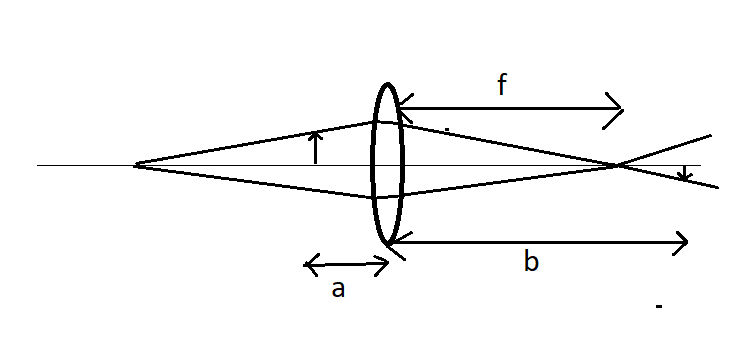
\includegraphics[height=0.3\textheight]{lens.png}
    \caption{Principskiss av en lins. Ett objekt avbildas på andra sidan, fast mindre.}
    \label{fig:lens}
\end{figure}
\subsection{Avbildningsfel}
I denna laboration diskuteras tre typer av avbildningsfel. Avbildningsfel skapar hinder vid design av optiska komponenter.
De tre typerna är:
\begin{itemize}
    \item Koma, där ljus som kommer in snett mot linsens optiska axel bryts olika mycket. Därmed skapas en utsmetad
    avbildning på andra sidan linsen. Se figur \ref{fig:got}f.
    \item Sfärisk aberration, som beror på att ljus som når sfäriska gränsytor inte bryts på samma sätt i kanten av linsen som paraxiala strålar.
    Strålarna som når kanten får en kortare brännvidd. Se figur \ref{fig:got}g.
    \item Kromatisk aberration, som beror på att glas med samma brytningsindex inte bryter ljus med olika våglängd
    likadant. Varje våglängd får därmed en egen fokalpunkt och bilden blir utsmetad. Se figur \ref{fig:got}h.
\end{itemize}
\section{Material och metod}
kollimera och linjera i separat dokument,  
Det fysiska materialet för denna laboration har endast varit en dator. Programvaran som tillhandahölls
av instutionen är Geometric Optics Tool för analys av optiska komponenter och MATLAB för dataanalys. 
Dessa program erbjöds av instutionen och därför fanns inte så mycket annat att välja på.

Arbetssättet i Geometrical Optics Tool (hädanefter förkortat som GOT) liknade det det skulle gjort
i en verklig laborationssal. Uppställningen sattes upp enligt instruktioner i programmet, 
resultat iakttogs och sedan dokumenterades uppställningen genom att ta en skärmdump av akutell uppställning.

För att mäta avlänkningsvinkeln i prismat användes programmet MB-Ruler som är en digital linjal
som kan mäta vinklar och avstånd på skärmen.

\section{Resultat}
\subsection{Beräkning av divergens}
Jag valde två punkter och avståndet $d_1 = 9.28, d_2 = 5.40, l = 7$.
Insättning i ekvation \ref{eq: div} gav en vinkel $\theta = \ang{31.28}$.

\subsection{Mätvärden från prismat}
Ljusets våglängd 555 nm. Alla mätvärden anges i grader.
\begin{table}[h]
    \begin{tabular}{|l|l|}
    \hline
    Infallsvinkel & Avlänkningsvinkel \\ \hline
    50.04         & 75.49             \\ \hline
    57.21         & 65.26             \\ \hline
    60.29         & 64.55             \\ \hline
    63.33         & 64.48             \\ \hline
    65.99         & 64.59             \\ \hline
    70.71         & 66.46             \\ \hline
    80.81         & 71.95             \\ \hline
    90            & 77.63             \\ \hline
    \end{tabular}
    \end{table}

Ljusets våglängd 700 nm. Alla mätvärden anges i grader.
\begin{table}[h]
    \begin{tabular}{|l|l|}
    \hline
    Infallsvinkel & Avlänkningsvinkel \\ \hline
    45.98         & 90                \\ \hline
    50.25         & 62.88             \\ \hline
    60.04         & 59.69             \\ \hline
    60.42         & 59.27             \\ \hline
    65.44         & 60.27             \\ \hline
    70.36         & 61.89             \\ \hline
    80.74         & 67.70             \\ \hline
    89.65         & 75.45             \\ \hline
    \end{tabular}
    
\end{table}
\pagebreak
\subsection{Uppställningar från GOT}

\begin{figure}[h!]
    \begin{tabular}{cc}
    \subfloat[Lins långt ifrån källan]{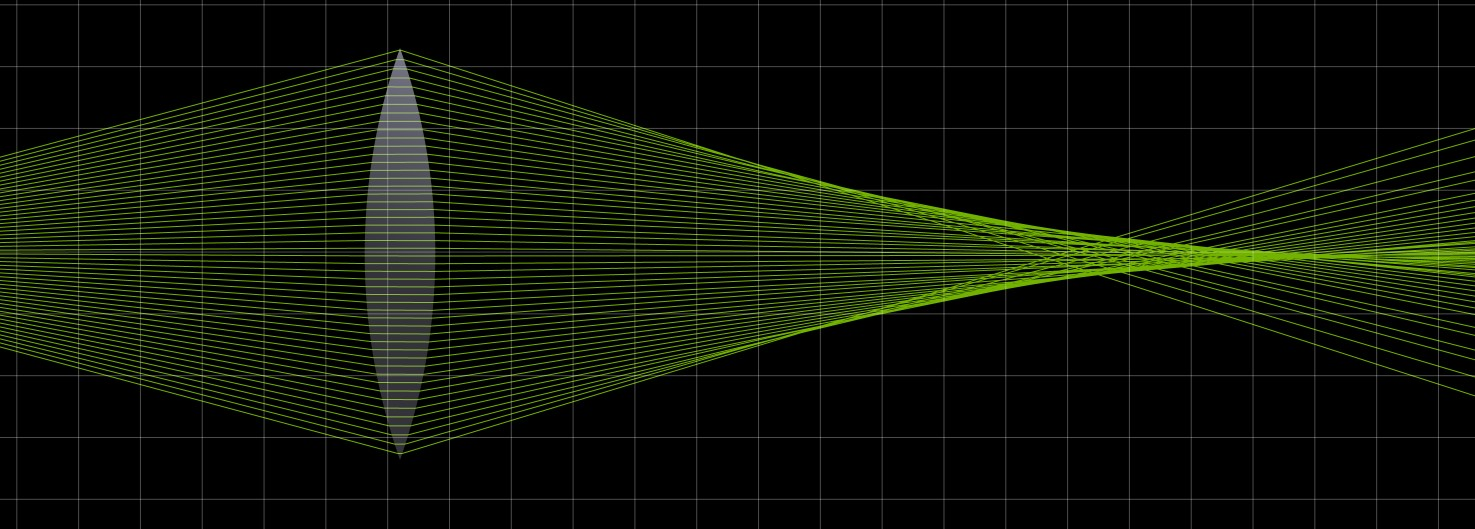
\includegraphics[width = 3in]{litenb.jpg}} &
    \subfloat[Lins nära källan]{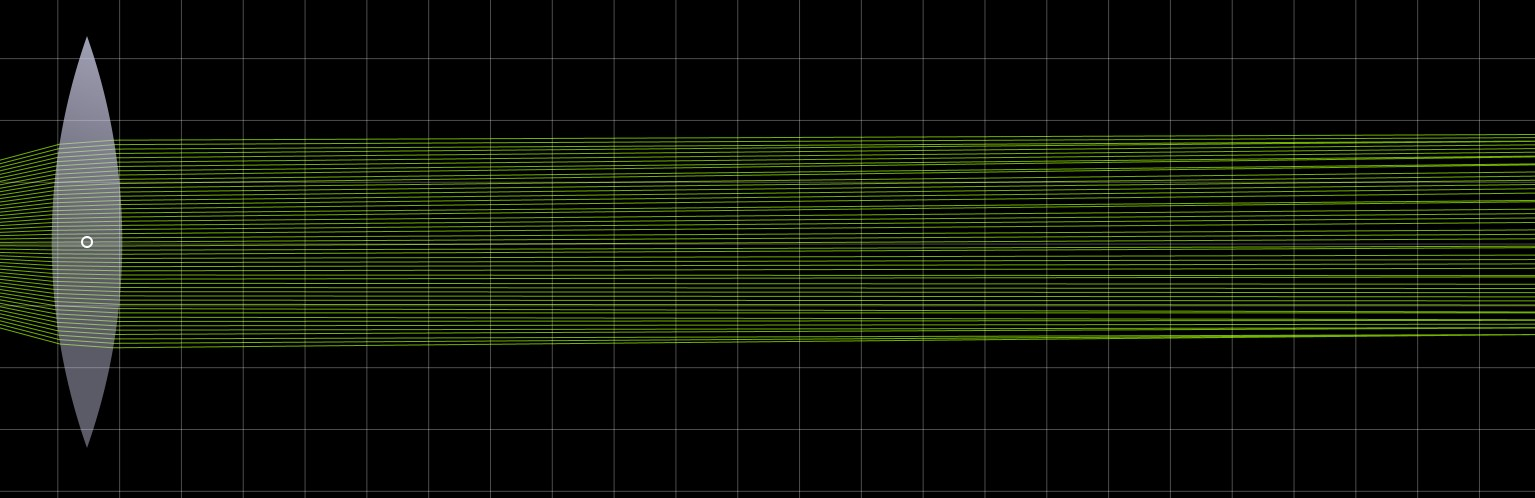
\includegraphics[width = 3in]{langb.jpg}}\\
    \subfloat[Sned lins]{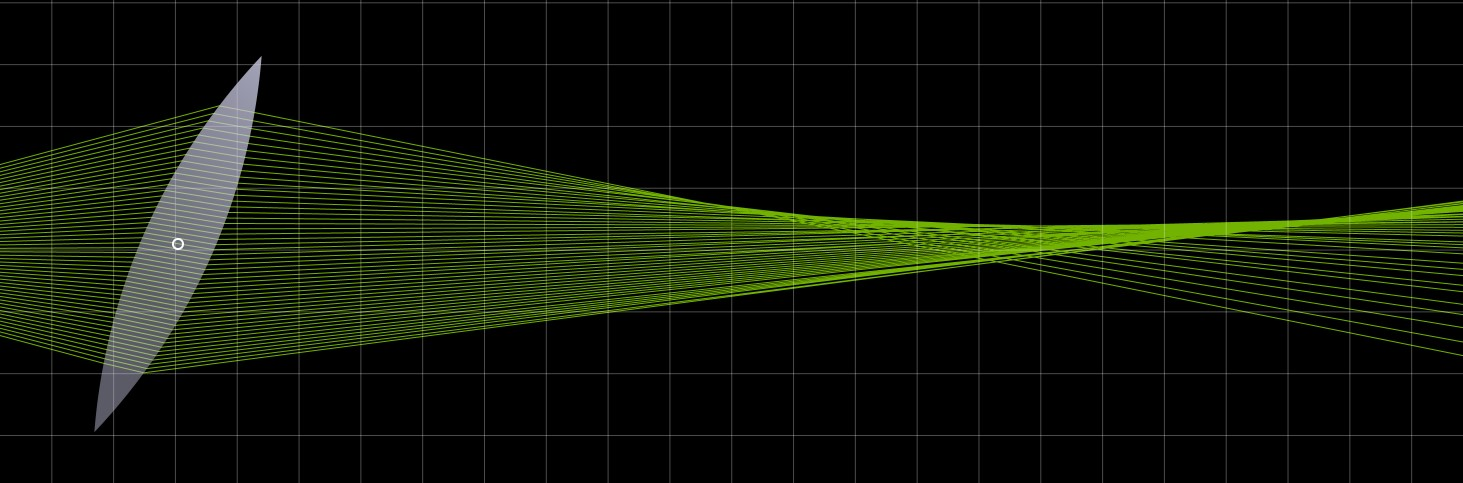
\includegraphics[width = 3in]{sned.jpg}} &
    \subfloat[Lins förskjuten i planet]{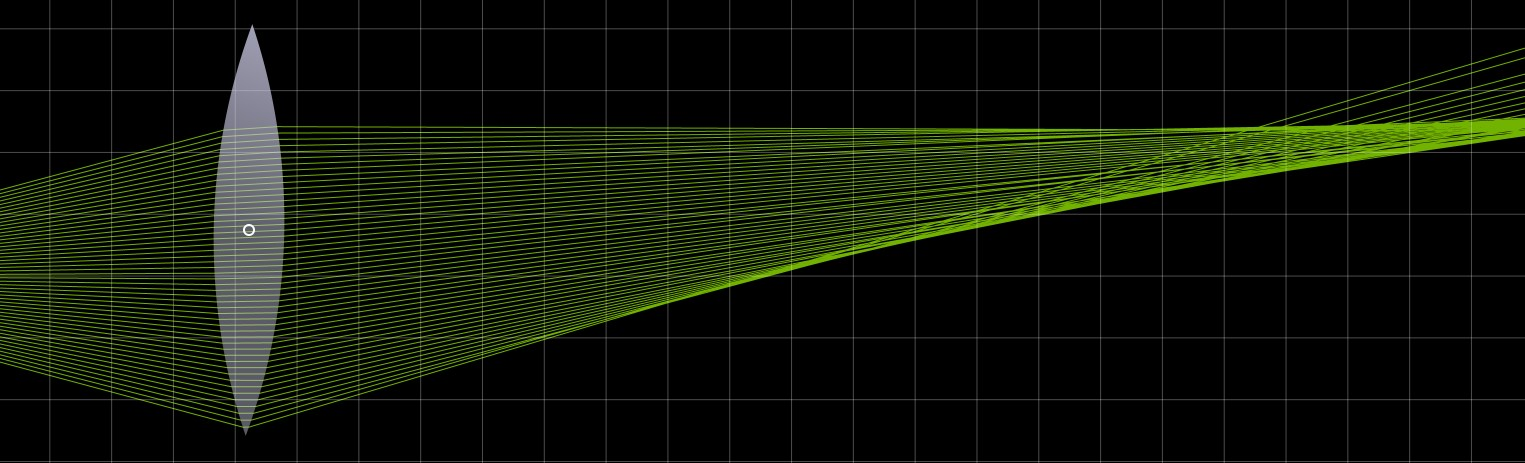
\includegraphics[width = 3in]{skev.jpg}}\\
    \subfloat[Ungefär samma avstånd till källan som brännpunkten.]{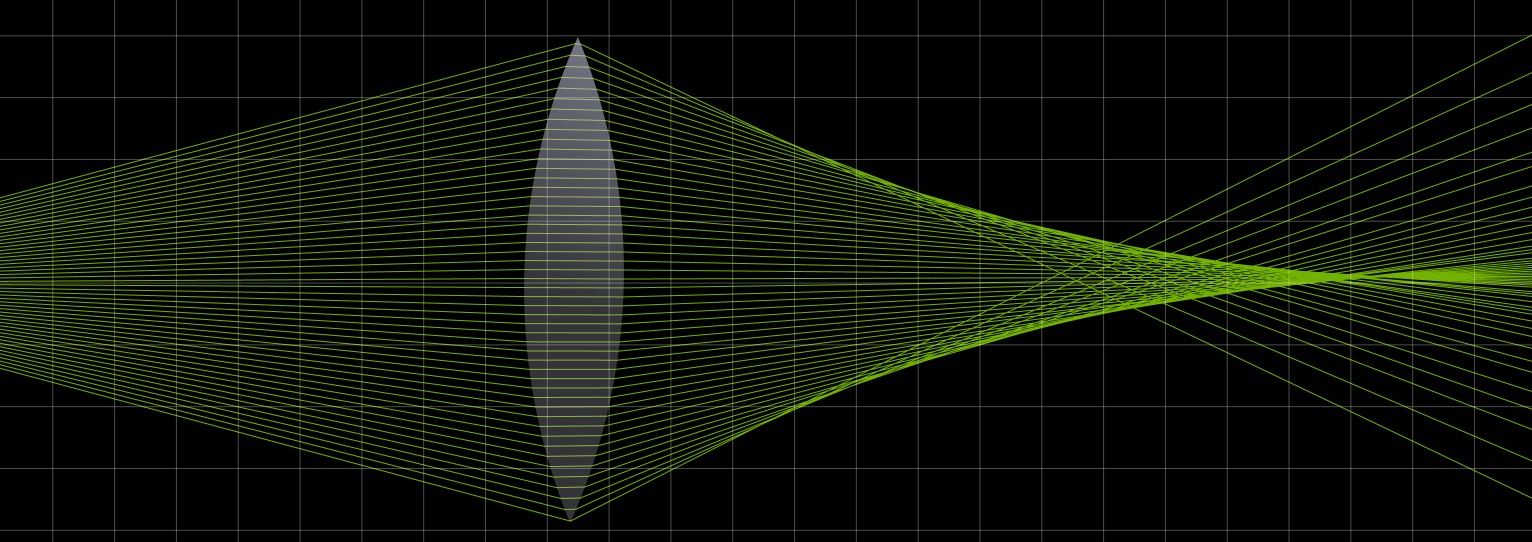
\includegraphics[width = 3in]{lika.jpg}} &
    \subfloat[Koma, ljuset kommer in snett och "smetas ut"]{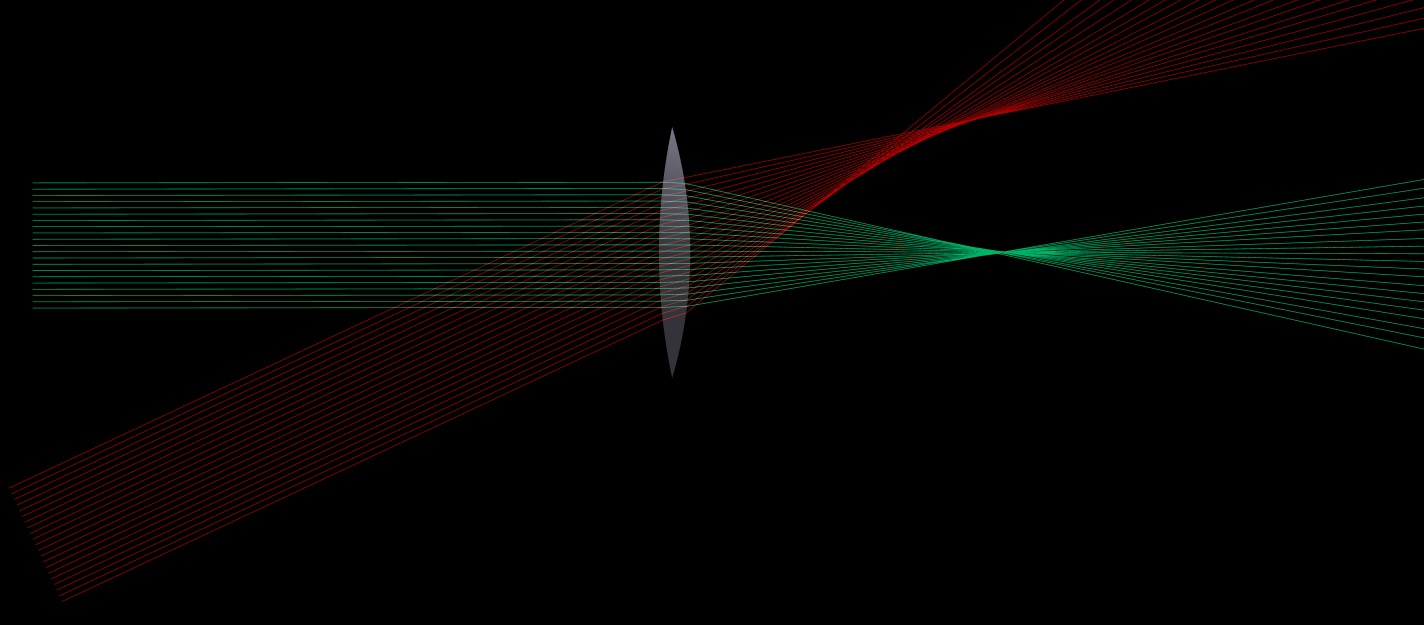
\includegraphics[width = 3in]{koma.jpg}}\\
    \subfloat[Sfärisk abherration, allt ljus fokuseras inte i brännpunkten.]{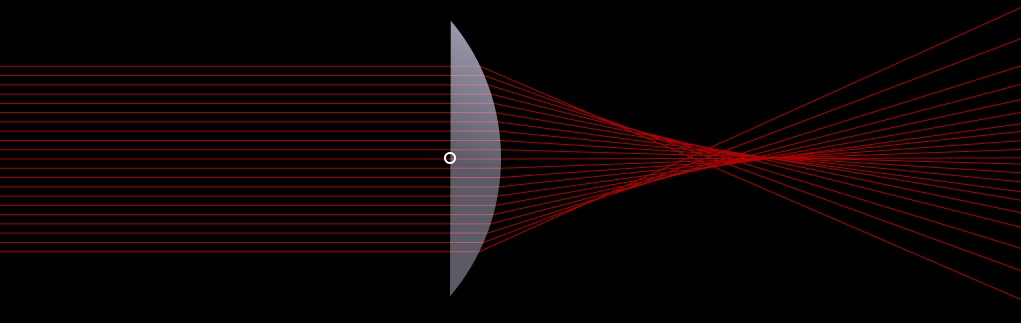
\includegraphics[width = 3in]{sphabherr.jpg}} &
    \subfloat[Kromatisk abherration, olika väglängder fokuseras på olika brännpunkter.]{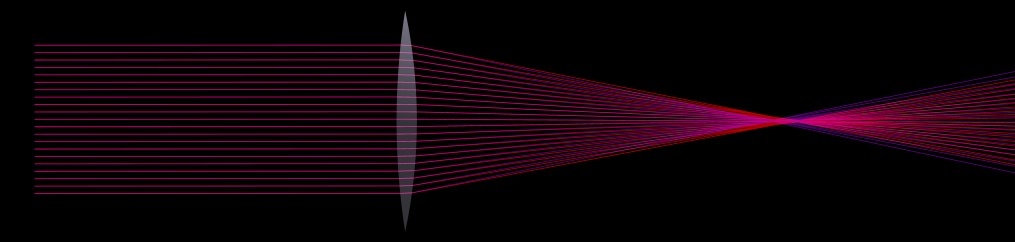
\includegraphics[width = 3in]{kromabherr.jpg}} \\
    \subfloat[Skarp brännpunkt]{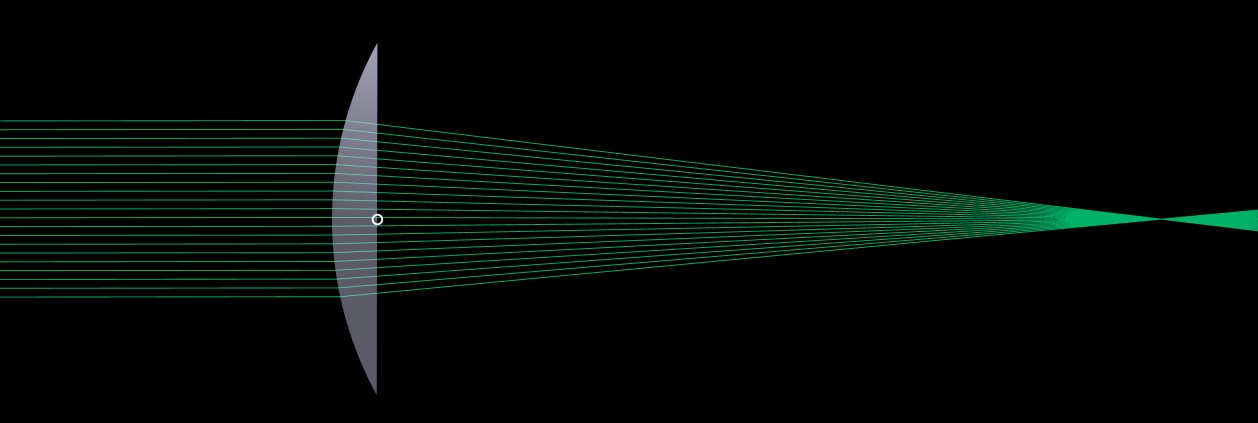
\includegraphics[width = 3in]{goodfocus.jpg}} &
    \subfloat[Oskarp brännpunkt]{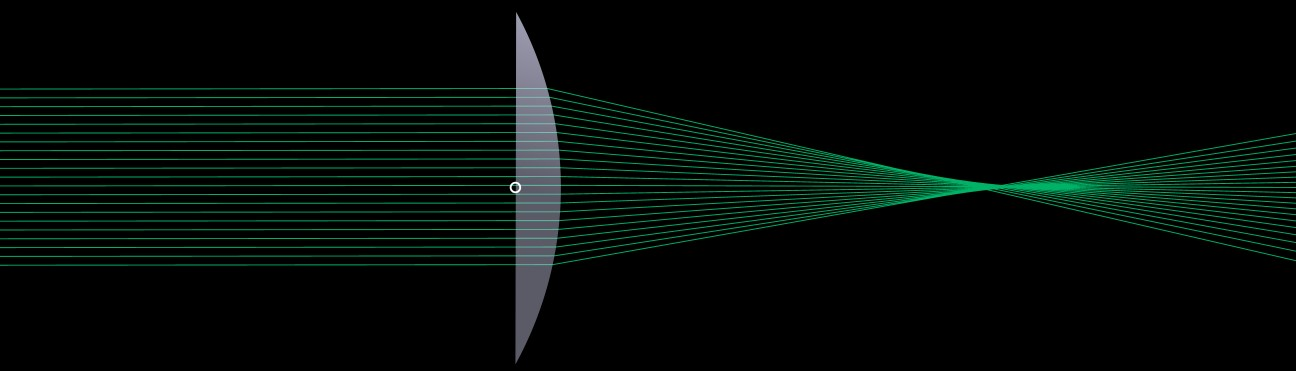
\includegraphics[width = 3in]{badfocus.jpg}} \\
    \subfloat[Totalreflektion i en rektangulär komponent.]{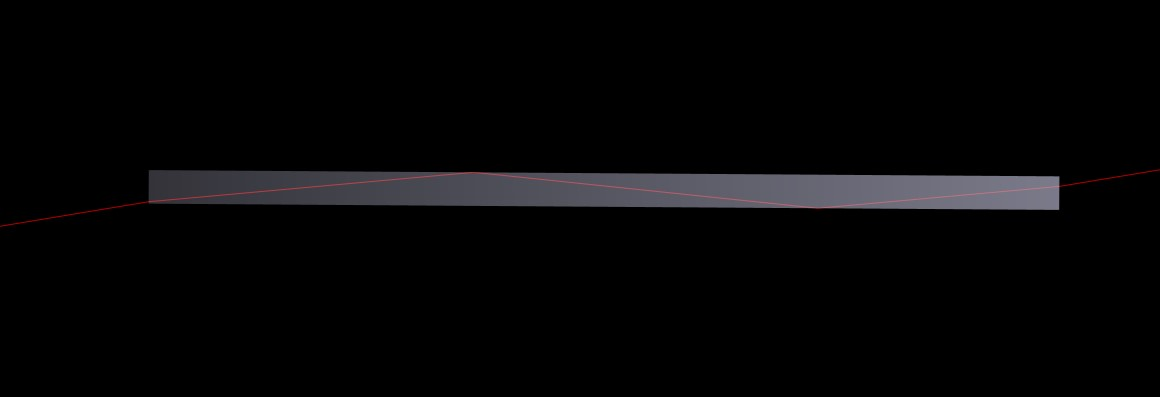
\includegraphics[width = 3in]{total.jpg}} 
    \end{tabular}
    \caption{De olika uppställningarna i GOT}
    \label{fig:got}
    \end{figure}

\pagebreak

\section{Diskussion och slutsatser}
\subsection{Linser}

\subsection{Prismat}
\begin{figure}[h]
    \caption{Mätvärden plottade och tredjegradspolynom anpassade till mätvärdena.}
    \centering
    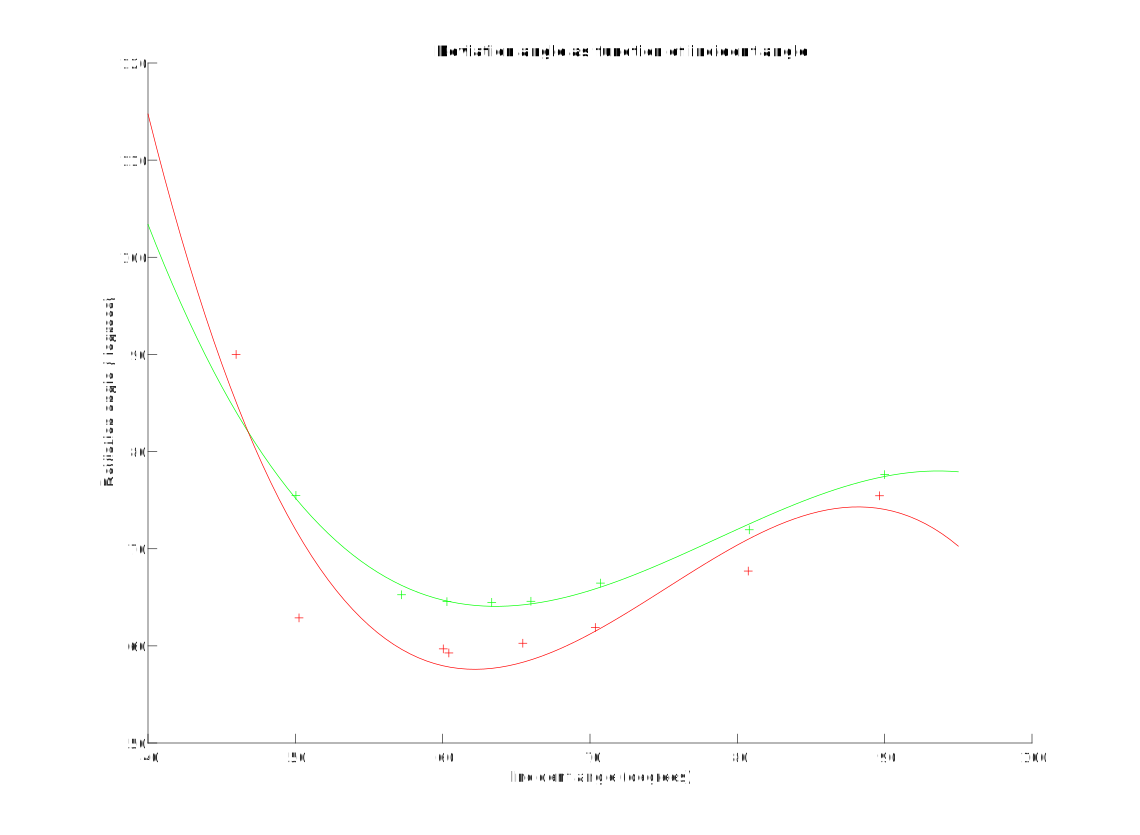
\includegraphics[width=\textwidth]{graph}
\end{figure}
vad var svårast att förstå, tips. vad kan mätfelen bero på.

\section{Referenser}
Våglära och Optik
Videor om kollimering och linjering. 

\section{Appendix A - Kollimering och linjering}
\subsection{Kollimering}
Kollimering (från latin: collimare - kasta i rak riktning)[wiki] innebär att man använder en konvex lins
för att parallellisera ljuset från en divergent ljuskälla. Detta görs genom att placera linsen
framför ljusstrålen, med fördel nära ljuskällan och justera avståndet till källan tills strålarna är parallella
på alla avstånd. En spegel kan användas så att ljuskälla och kollimeringspunkt hamnar bredvid varandra. Se figur \ref{fig:kollimering}.
Genom att placera linsen nära ljuskällan ser vi till att brännvidden blir oändlig.
\begin{figure}[h]
    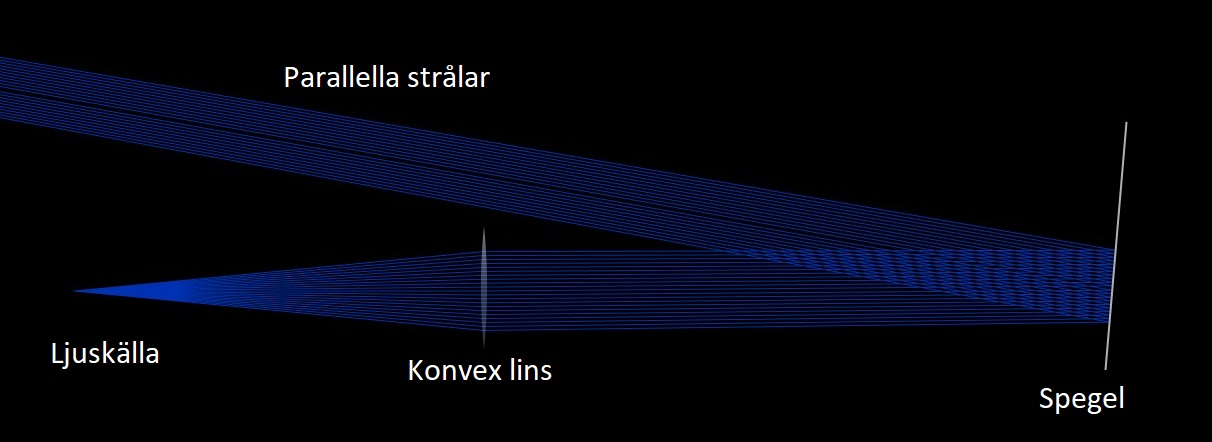
\includegraphics[width=\textwidth]{kollimera3.jpg}
    \caption{Kollimering av en divergent ljusstråle.}
    \label{fig:kollimering}
\end{figure}
\subsection{Linjering}
Att linjera lasern innebär att man tar en parallelliserad ljuskälla, exempelvis en laserstråle och ser till att det går igenom två bländare med rakast möjliga väg.
Detta görs genom att placera ut två speglar, en så nära den första bländaren som möjligt, och en så att ljusstrålen böjs ned mot den andra spegeln. Se figur \ref{fig:linjering}
Sedan justeras spegel 1 i figuren så att ljuset passerar igenom första bländaren så centralt som möjligt. Sedan används spegel 2 för att se till att hela ljusstrålen passerar
genom den vänstra bländaren.
\begin{figure}[h]
    \centering
    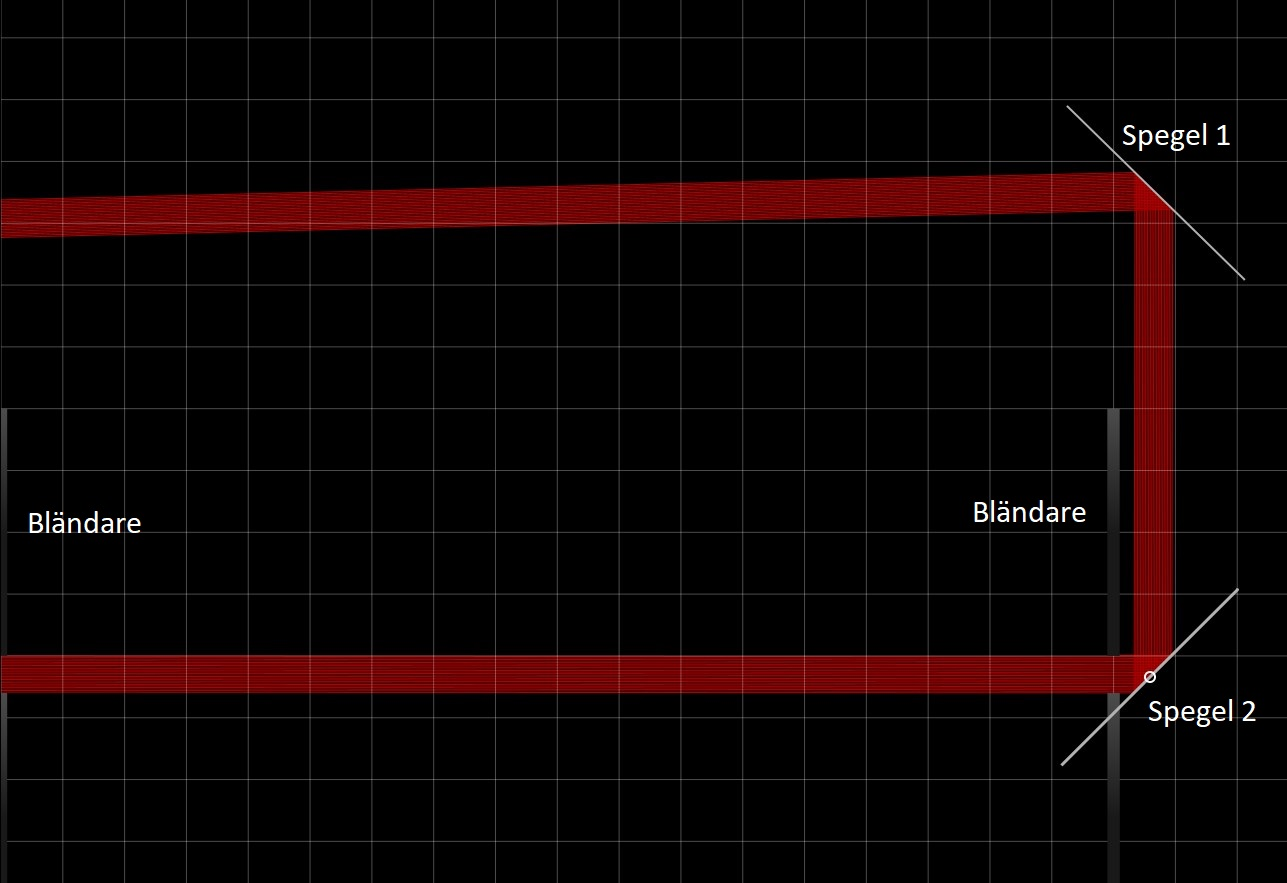
\includegraphics[width=0.6\textwidth]{linjera4.jpg}
    \caption{Kollimering av en divergent ljusstråle.}
    \label{fig:linjering}
\end{figure}
\pagebreak
\section{Övriga appendix}

\section{Anteckningar}

\subsection{Brännvidd}
När linsen placeras närmare ljuskällan ökar brännvidden för att till slut bli oändlig. Ju närmare jag placerar linsen,
ju mindre verkar brännvidden bli. Genom att rotera linsen förskjuter vi brännpunkter och
det bildas inget tydligt fokus. Genom att flytta linsen i samma plan böjs ljusstrålarna
olika mycket och vi får en förflyttning av brännpunkten.

Sätter vi $a = b = cf$ i $ \frac{1}{a} + \frac{1}{b} = \frac{1}{f}$ får vi $c=2$ alltså $a=b=2f$. Avståndet är alltså två brännvidder.


\subsection{Prismat}
Mätte vinklar, se tabell. Anpassade tredjegradspolynom och får minsta avlänksningsvinkel $\delta = 64.0680, \lambda=555$.

För $\lambda = 700$ fås analytiskt minimum $\delta = 57.5861$ men det sanna minimat ligger nog runt $60 grader$.
\end{document}
